\section{Sesión 16}

\subsection{Norma del supremo}

\begin{definicion}
	Sea $X$ un espacio métrico y sea $C(x)$ el conjunto de todas las funciones continuas y acotadas sobre $X$. Para $f\in C(x)$ se define: 
	$$\|f\|=\sup_{x\in X}|f(x)|,$$
	que se denominan la norma del supremo de $f$ sobre $X$. 
	\begin{enumerate}
		\item Como $f$ es acotada $\implies |f(x)|<\infty, \forall x\in X$. Además, $\|f\|=0\iff f(x)=0$. 
		\item Si $h=f+g\implies |h(x)|\leq |f(x)|+|g(x)|\implies \|f+g\|\leq \|f\|+\| g\|$. 
		\item Si $f,g\in C(X)\implies$ se define $d(f,g):=\|f-g\|$. 
		\item Lenguaje: En algunas casos a los cerrados de $C(x)$ se les llama uniformemente cerrados y a la cerradura de $A\subset C(X)$ se le llama cerradura uniforme. 
	\end{enumerate}
\end{definicion}

\subsubsection{Convergencia}
Sea $(x,+,\cdot, \mathbb{R})$ es un espacio vectorial. 

\begin{definicion}
	Una función $\|\cdot\|: X\to [0,\infty)$ es una norma sobre $X$, si:
	\begin{enumerate}
		\item $\|x+y\|\leq \|x\|+\|y\|,\quad \forall x,y\in X$. 
		\item $\|\lambda x\| =|\lambda| \cdot \|x\|,\quad \forall x\in X, \forall \lambda\in \mathbb{R}$
		\item $\|x\|=0\iff x=0$. 
	\end{enumerate}
Al par $(x,\|\cdot\|)$ se le dice espacio normado. 
\end{definicion}

\begin{definicion}
	Una sucesión $(x_n)\subset X$ converge a $x\in X$, si $\|x_n-x\|\to  0$.
\end{definicion}

\begin{definicion}
	Una sucesión $(x_n)\subset X$ es de Cauchy si $\forall \varepsilon >0\exists N\in \mathbb{Z}^+\ni$ si $n,m\geq N\implies \|x_n-x_m\|<\varnothing$. 
\end{definicion}

\begin{definicion}
	Sea
	\begin{enumerate}
		\item Se dice que $X$ es \textbf{completo} si toda sucesión de Cauchy es convergente. 
		\item Un espacio vectorial normado y completo es un espacio de Banach. 
		\item Un espacio vectorial de Banach tal que la norma se obtiene un producto interno ($\|x\|:=\sqrt{\rangle x, x\langle}$), es un espacio de Hilbert. 
		\end{enumerate}
\end{definicion}

\begin{definicion}
	Sea $f$ una función definida en $A\subset \mathbb{R}$, la norma del supremo (norma uniforme) es el número sobre $\overline{\mathbb{R}}$, $\|f\|_\infty:= \sup\{|f(x)|:x\in A\}$
\end{definicion}

\begin{nota}
	Una sucesión $(x_n)$ de elementos en $\overline{\mathbb{R}}$ converge a $x\in\mathbb{R}$ si $\exists N\in\mathbb{Z}^+\ni x_n$ es finito si $n\geq N$ y si la sucesión de reales $(x_n)$ converge a $x$. 
\end{nota}

\begin{prop}
	Sea $(f_n)$ una sucesión de funciones definidas en $A\subseteq \mathbb{R}$ y $f$ una función definida en $A$. Los enunciados siguientes son equivalentes:
	\begin{enumerate}
		\item $(f_n)$ converge uniformemente. 
		\item La sucesión ($\|f_n-f\|_\infty$) sobre $\overline{\mathbb{R}}$ converge a 0. 
	\end{enumerate}
\end{prop}

\begin{teorema}(Criterio de Cauchy uniforme)
	Sea $(f_n)$ una sucesión de funciones definidas sobre un conjunto $A\subset \mathbb{R}$. Los enunciados siguientes son equivalentes: 
	\begin{enumerate}
		\item $(f_n)$ converge uniformemente a una función $f(x)$.
		\item Dado $\varepsilon>0\exists N\in\mathbb{Z}^+\ni$ si $m,n\geq N$, entonces $|f_n(x)-f_m(x)|<\varepsilon, \forall x\in A$. 
		\item Dado $\varepsilon>0\exists N\in\mathbb{Z}^+\ni$ si $m,n\geq N\implies \|f_n-f_m\|_\infty<\varepsilon$. 
	\end{enumerate}
\end{teorema}

\begin{teorema}
	Sea $(f_n)$ una sucesión de funciones definidas sobre $A\subset \mathbb{R}$ que converge uniformemente a la función $f$ definida sobre $A$. Si cada $f_n$ continua en $c\in A\implies f$ es continuas en $c\in A$. 
\end{teorema}

\begin{teorema}(Dini)
	Sea $(f_n)$ una sucesión de funciones continuas en un intervalo cerrado y acotado $I$. Suponga $(f_n)$ converge puntualmente a una función continua $f$ y que $(f_n)$ es monótona. Entonces, $(f_n)$ converge uniformemente a $f$. 
	
	$$\overbrace{f_n}^{\text{continua}}\xrightarrow{\text{puntual sobre compacto}}\overbrace{f}^{\text{continua}}+\textcolor{red}{(f_n)\text{es monótona}}\implies f_n\xrightarrow{\text{unif}}f$$

\end{teorema}

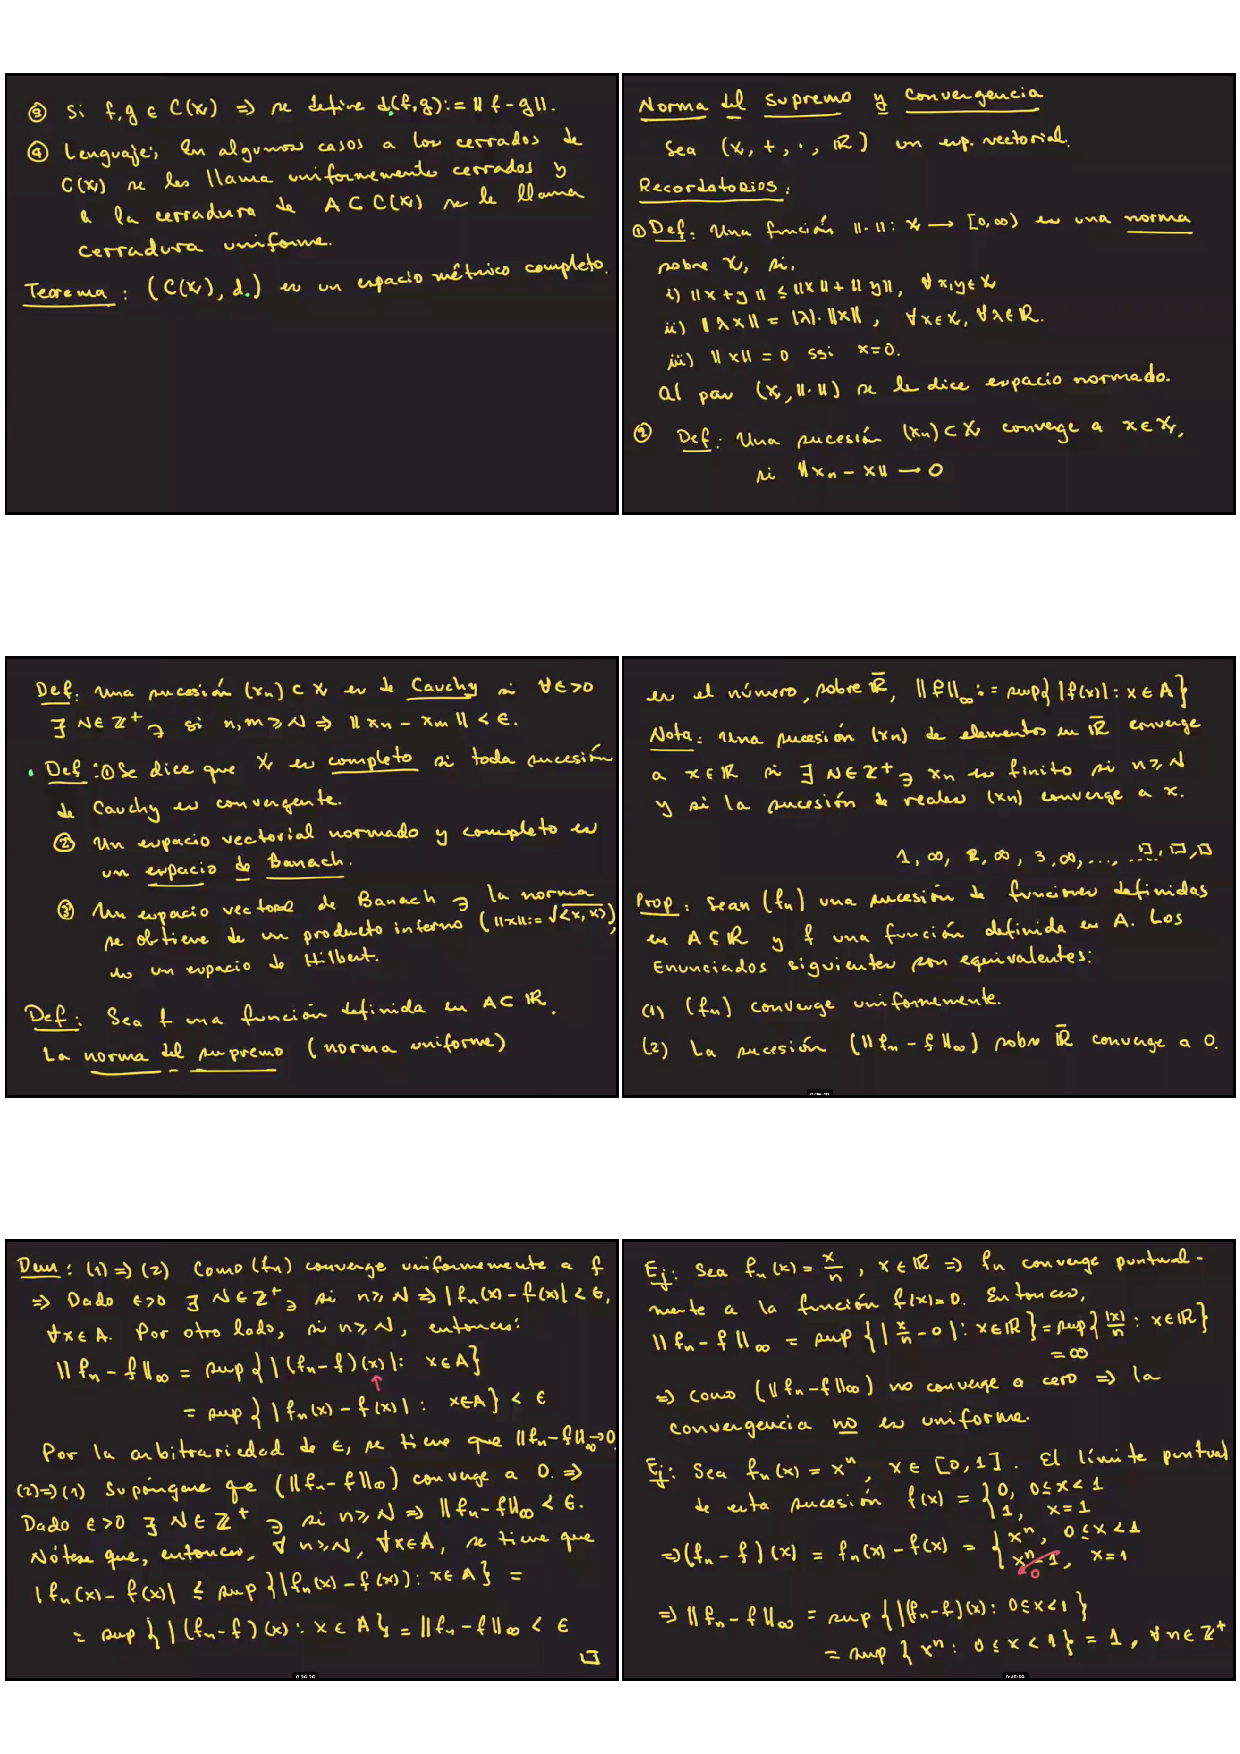
\includepdf[pages=-]{apendices/s16.pdf}